\section{Results and Discussion}
\label{sec:results}

This section interprets the verified experimental outcomes established on the historical 2016--2018 held-out test partition. Table~\ref{tab:model_performance} summarizes the primary performance metrics for the evaluated architectures.

\subsection{Overall Multi-Hazard Performance}
A consistent pattern emerges across the three evaluated hazards under the chronological evaluation protocol. The selected Random Forest Flood model exhibits moderate discriminatory performance with a recall-oriented predictive boundary. In contrast, the leakage-remediated LightGBM Heatwave model demonstrates high discriminatory performance under the evaluated test distribution. Predicting Compound risk remains substantially more difficult, as the simultaneous occurrence of extreme interacting hazards is inherently rarer and dynamically more complex. Due to the significant class imbalance across all hazards, evaluation heavily prioritizes ROC-AUC and PR-AUC simultaneously.

\subsection{Flood Prediction Results}

\begin{figure}[t]
\centering
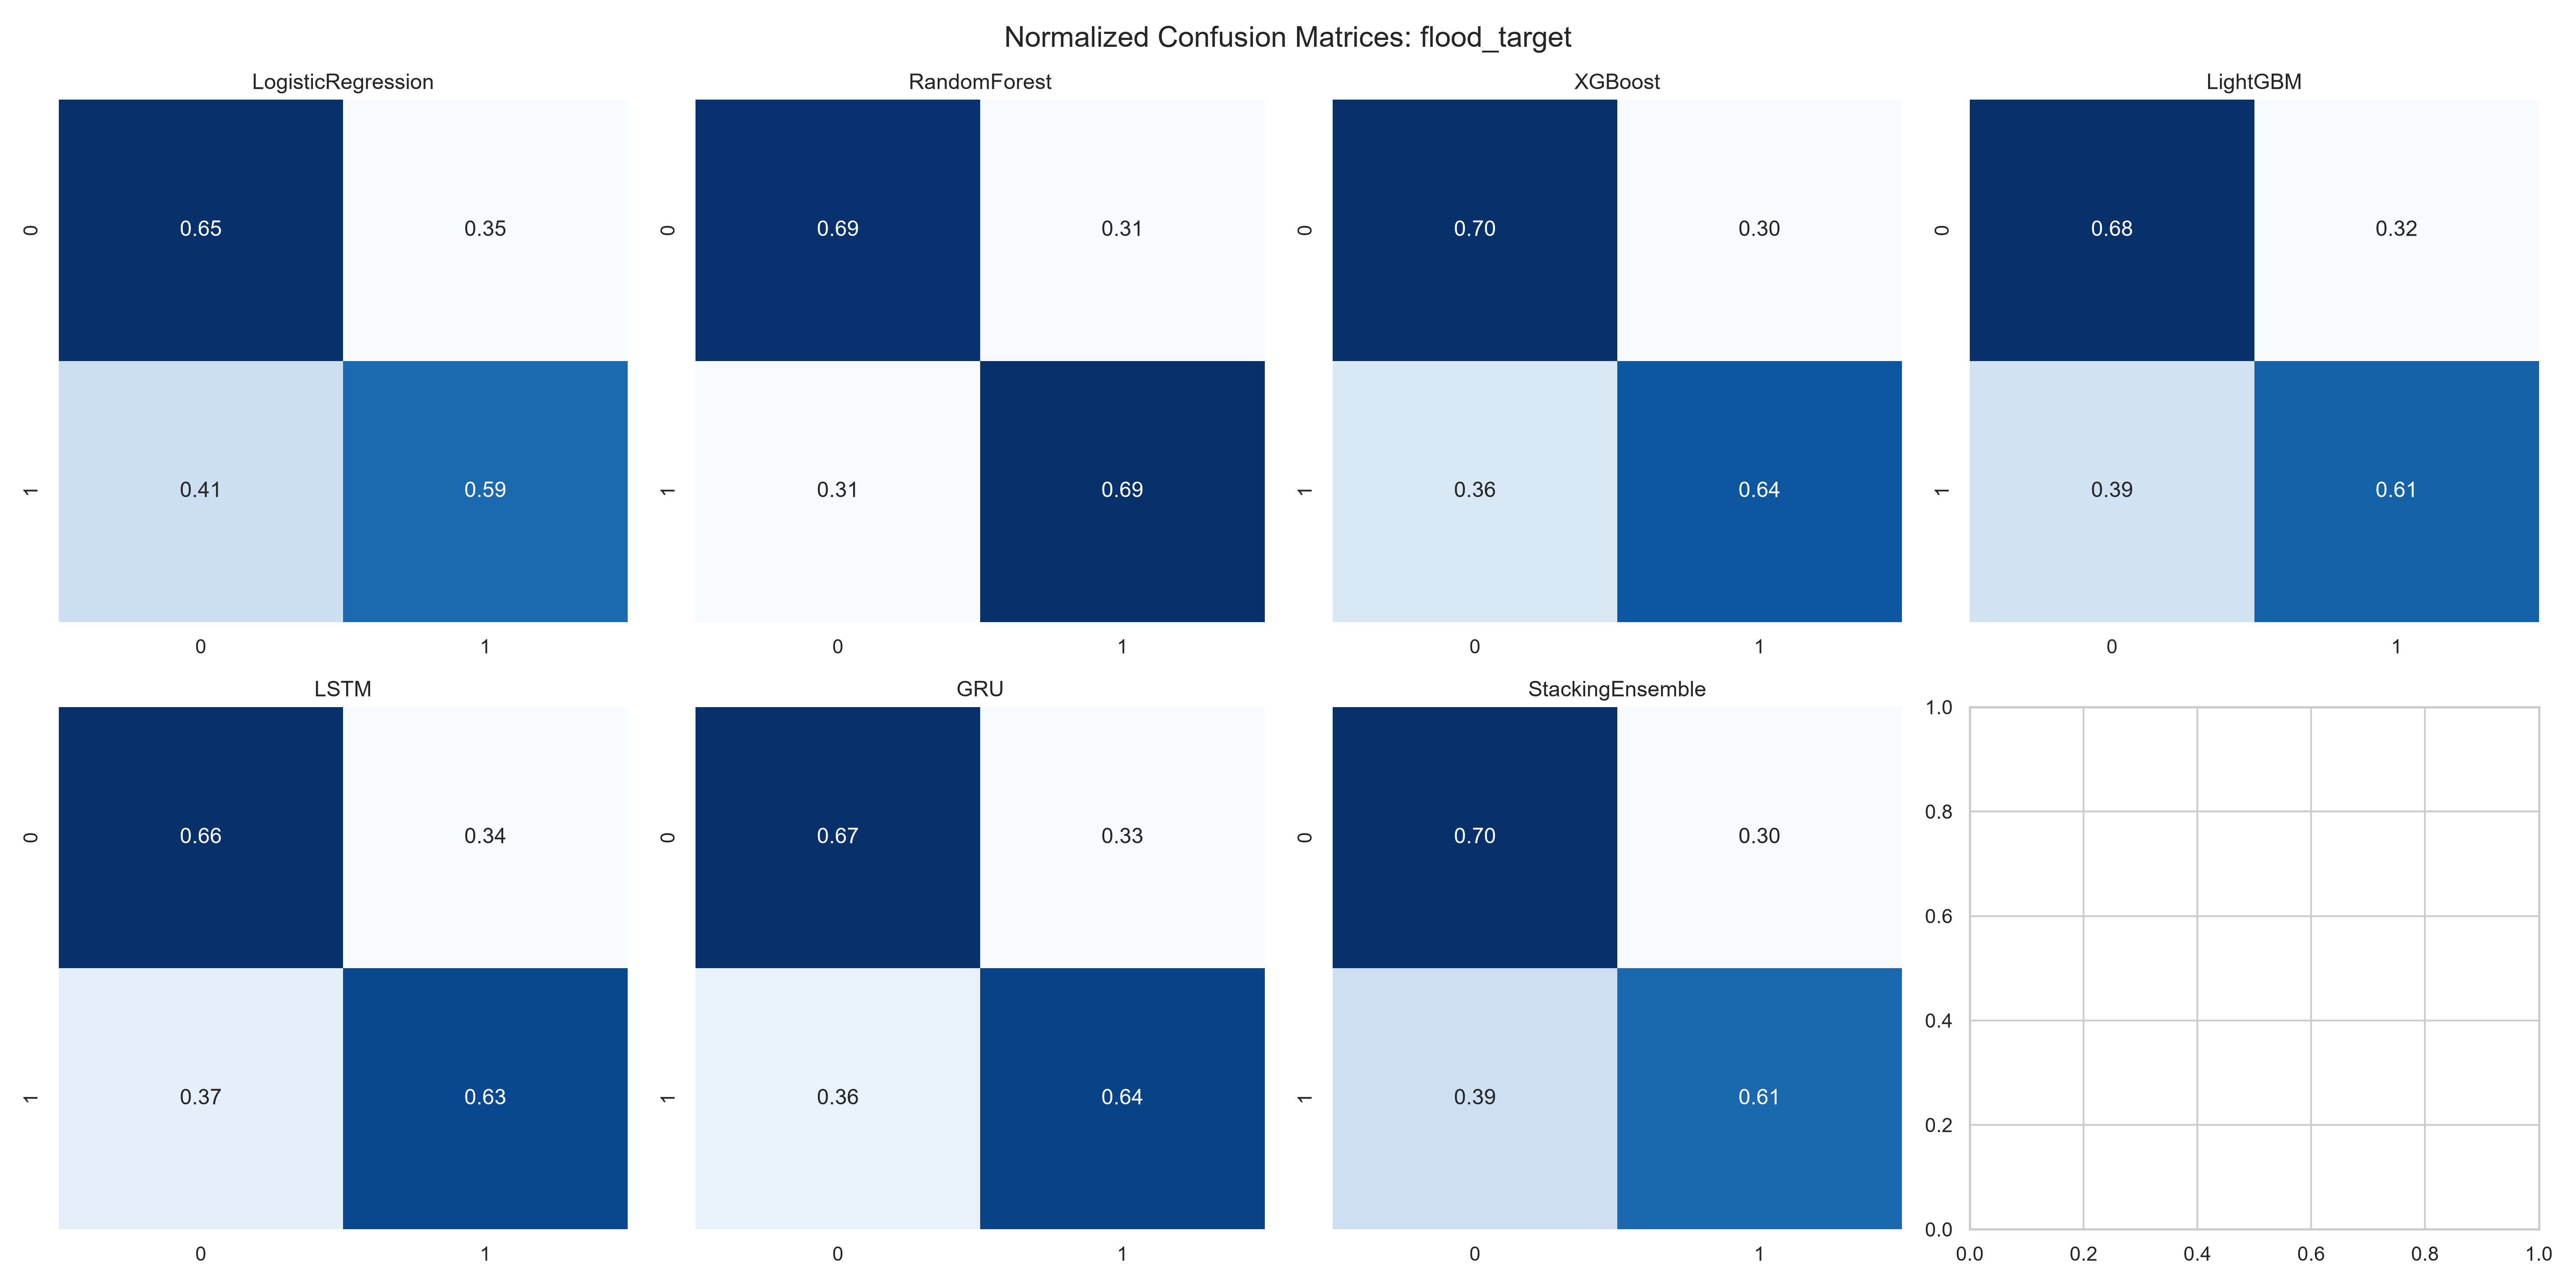
\includegraphics[width=\columnwidth]{figures/Fig02_Flood_Confusion_Matrix.png}
\caption{Normalized confusion matrix for the Random Forest flood-risk classifier on the chronological 2016--2018 test set.}
\label{fig:flood_confusion}
\end{figure}
The operational Random Forest model for Flood prediction achieves an Accuracy of 69.16\%, an $F_1$-score of 0.4686, an ROC-AUC of 0.7184, and a PR-AUC of 0.3468, yielding a final uncalibrated Brier Score of 0.2391. Most notably, the model achieves considerably higher Recall (69.30\%) than Precision (35.39\%). A higher recall indicates greater sensitivity to positive flood events, while the lower precision indicates a relatively high false-alarm burden. For early-warning applications, missed events and false alarms represent distinctly different operational costs. The current configuration favors detecting true emergencies over minimizing false positives, establishing a pragmatic precision-recall trade-off rather than an assumed universal optimum. The specific classification outcomes are illustrated in the associated confusion matrix (Fig.~\ref{fig:flood_confusion}).

\subsection{Heatwave Prediction Results}

\begin{figure}[t]
\centering
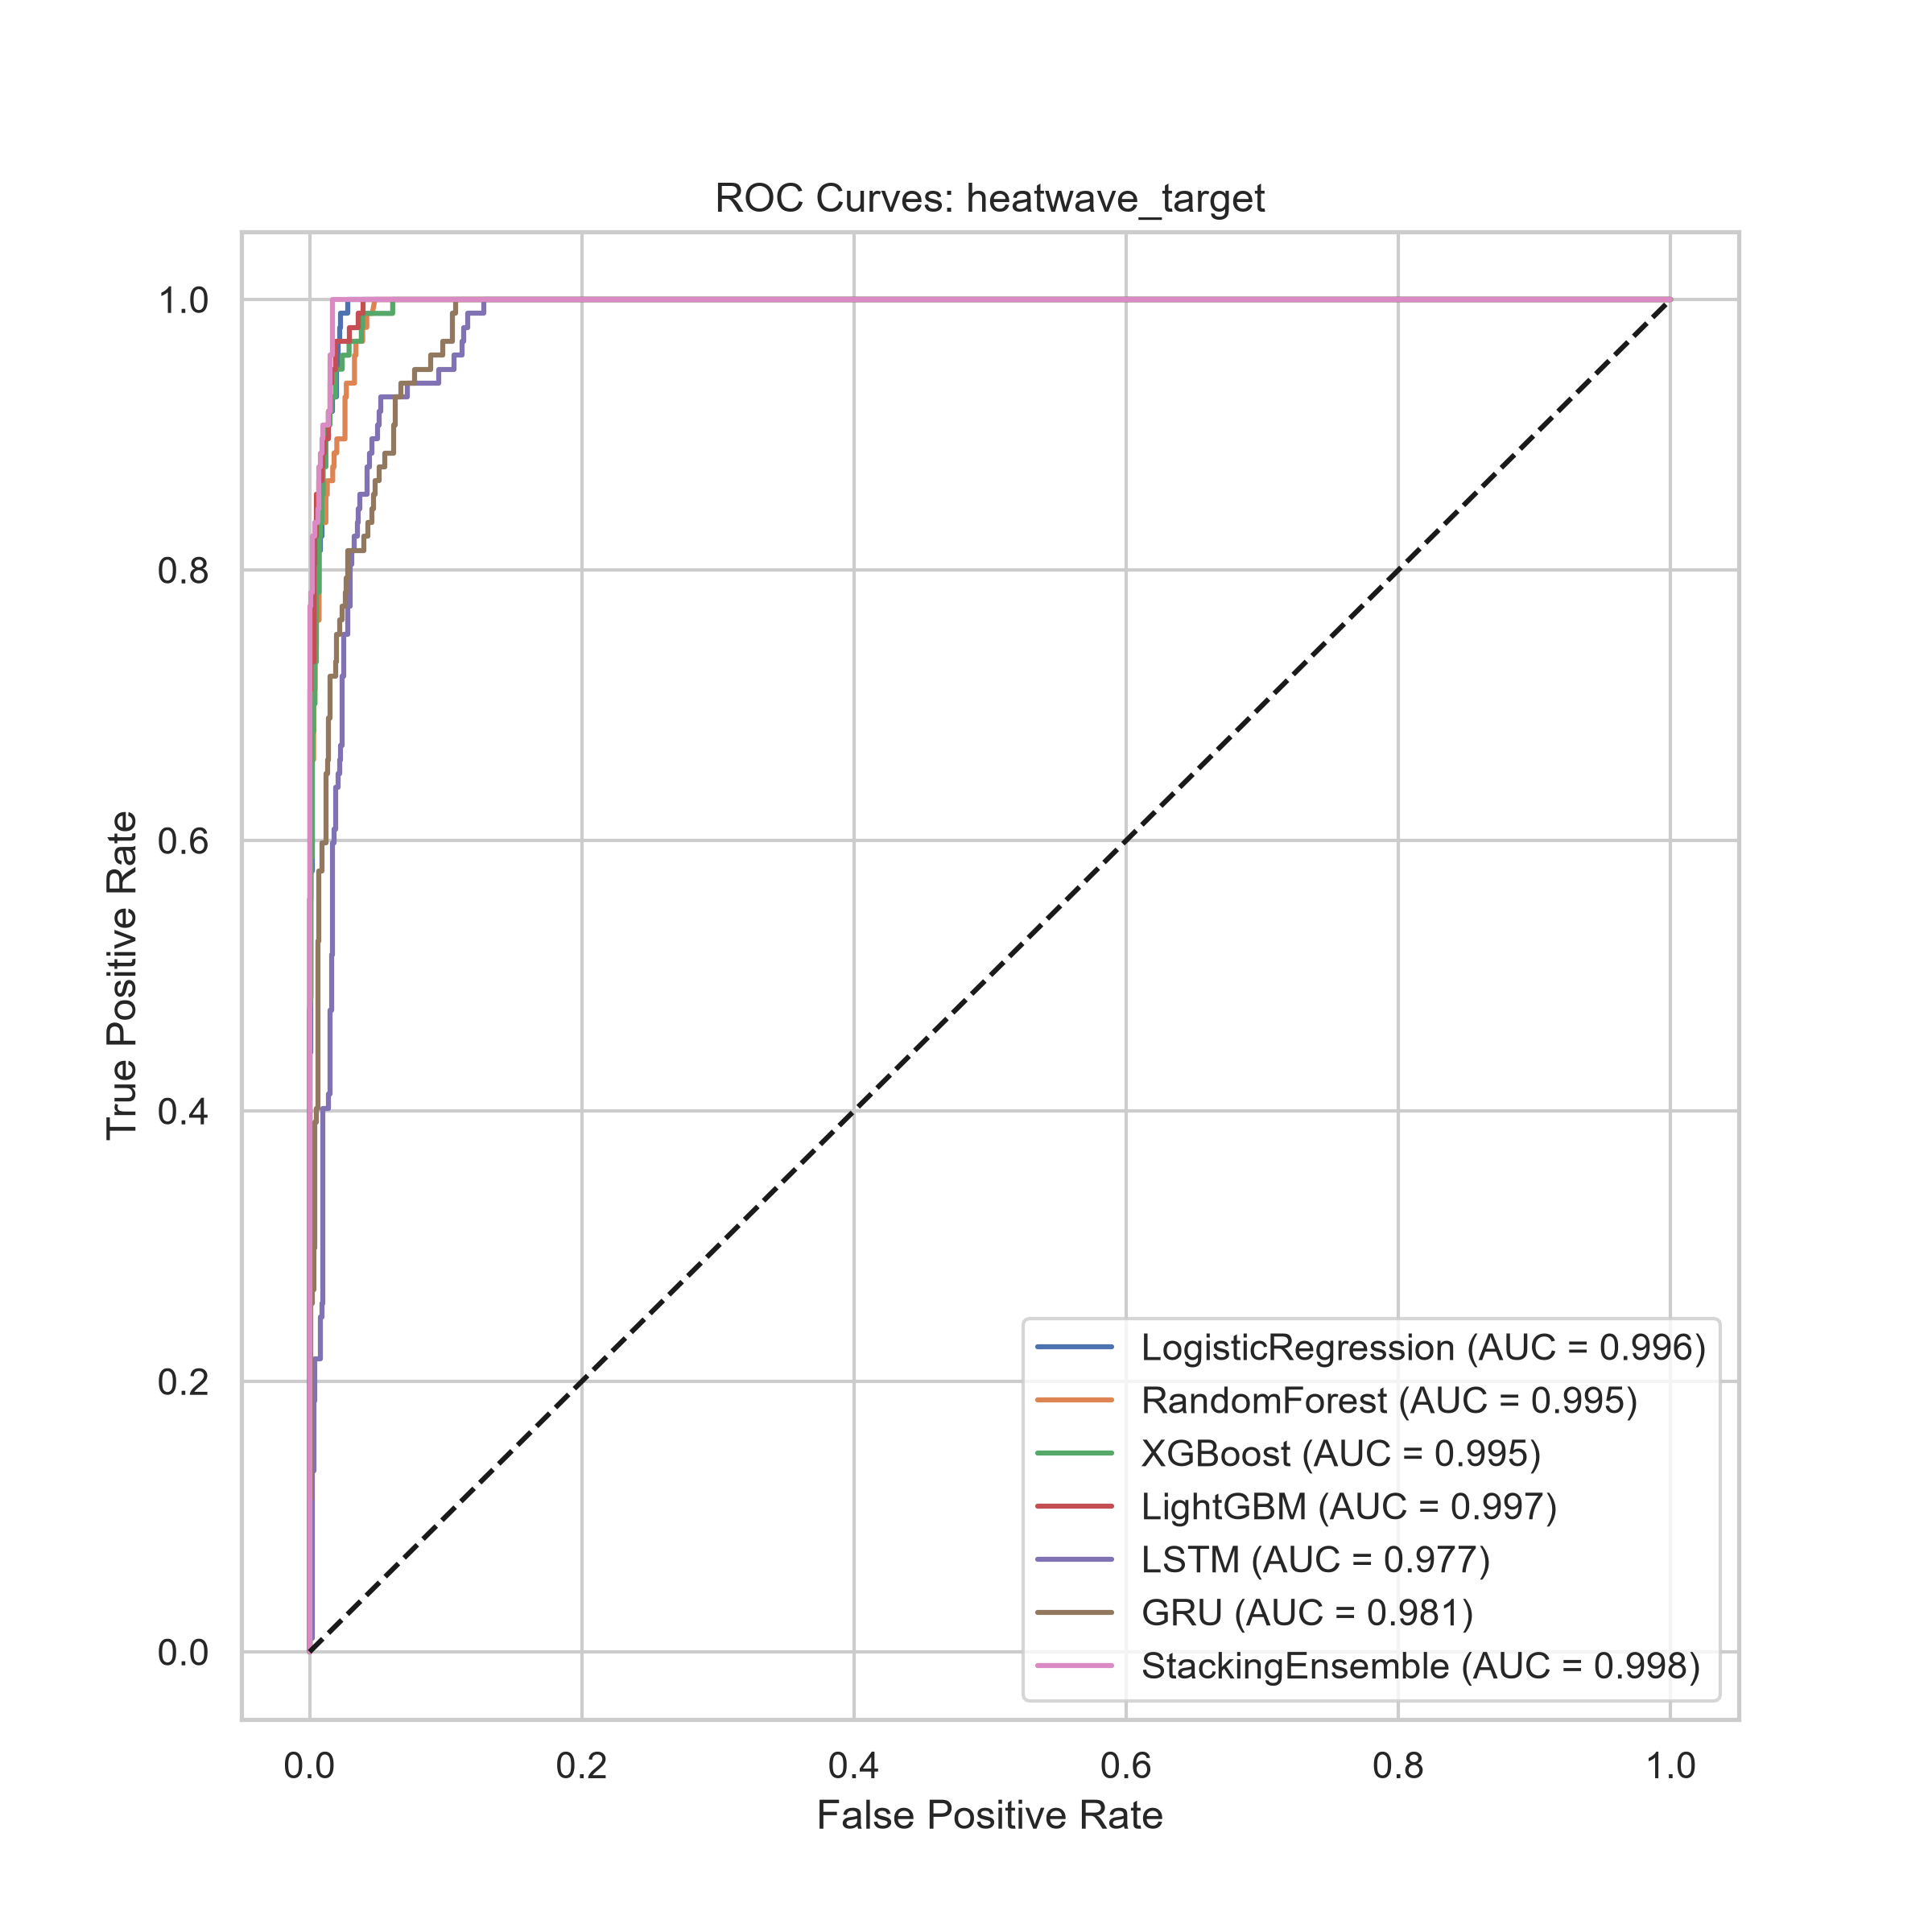
\includegraphics[width=\columnwidth]{figures/Fig03_Heatwave_ROC.png}
\caption{ROC curve for the leakage-remediated LightGBM heatwave classifier evaluated on the 2016--2018 held-out test set.}
\label{fig:heatwave_roc}
\end{figure}
The operational LightGBM model evaluating the Heatwave hazard demonstrates strong discrimination on the held-out 2016--2018 period. The model achieves an Accuracy of 97.99\%, Precision of 87.88\%, Recall of 89.69\%, an $F_1$-score of 0.8878, an ROC-AUC of 0.9969, and a PR-AUC of 0.9711, with a Brier Score of 0.0149. The associated ROC curve (Fig.~\ref{fig:heatwave_roc}) visually confirms this robust discrimination under the held-out test distribution. Critically, these results are derived exclusively from the leakage-remediated 41-feature configuration. The initial model iteration relied on deterministic proxy variables directly associated with the target definition; following their explicit removal, the model retained its performance, ensuring that predictions map underlying drivers rather than tautological indicators. 

\subsection{Compound-Risk Results and Operational Selection}
Predicting Compound hazards requires differentiating offline theoretical capacity from operational deployment feasibility (Table~\ref{tab:op_selection}). The GRU offline benchmark achieved the strongest predictive discrimination for the Compound target, recording an $F_1$-score of 0.4343, an ROC-AUC of 0.9598, and a PR-AUC of 0.4838. In comparison, the Logistic Regression Stacking Ensemble achieved an $F_1$-score of 0.3419, an ROC-AUC of 0.9495, and a PR-AUC of 0.3891. 

Despite the stronger offline predictive performance of the GRU, it inherently requires an $(N, 14, 45)$ temporal tensor, representing a 14-day sequence of 45 standardized features. Conversely, the ClimateGuardian AI realtime predictor is explicitly designed around stateless, point-in-time feature vectors and avoids maintaining a recurrent 14-day sequence buffer to minimize live-system latency. Consequently, the Stacking Ensemble is explicitly retained as the operational Compound architecture. Thus, the Stacking Ensemble should be interpreted as the deployment-oriented choice rather than the numerically dominant offline Compound model.

\subsection{Lead-Time Performance}

\begin{figure}[t]
\centering
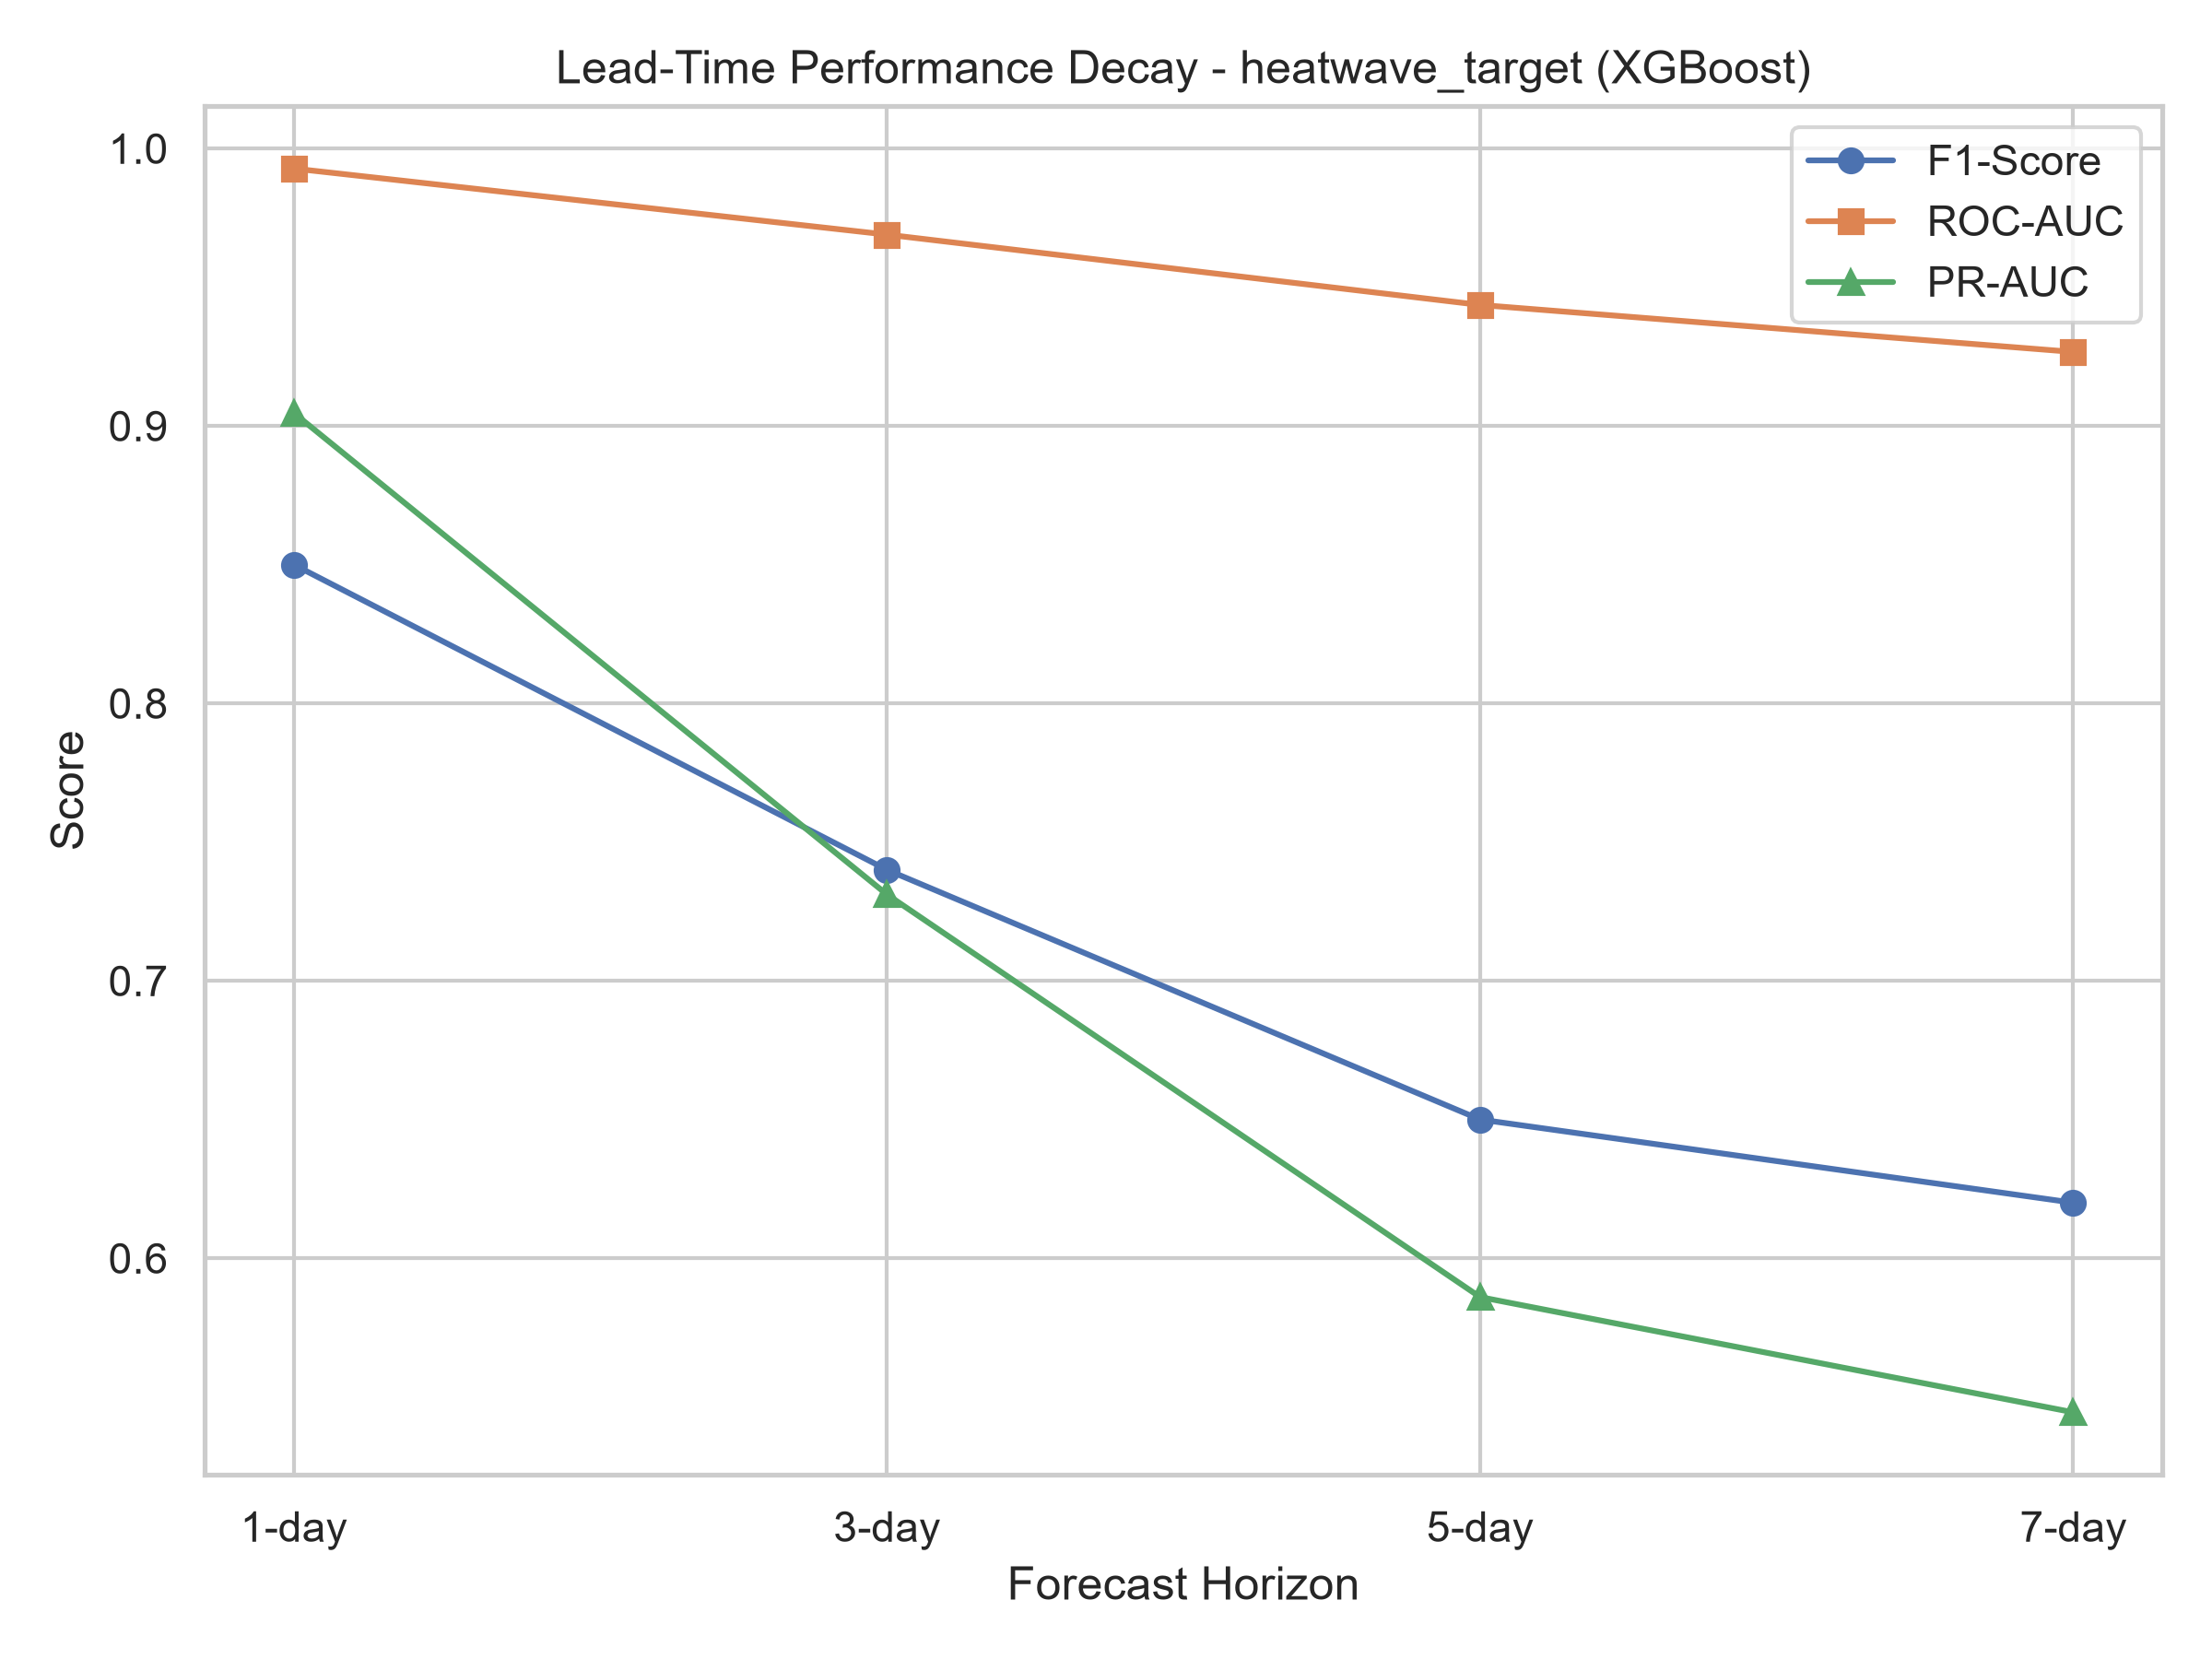
\includegraphics[width=\columnwidth]{figures/Fig06_Heatwave_LeadTime.png}
\caption{Heatwave F1-score degradation across the evaluated 1-, 3-, 5-, and 7-day lead-time horizons.}
\label{fig:heatwave_leadtime}
\end{figure}
Evaluating predictive degradation over future horizons is critical for early-warning mechanisms. Utilizing target-shifting, the lead-time experiment quantified Heatwave prediction viability at extended horizons (Fig.~\ref{fig:heatwave_leadtime}). Predictive performance logically declines as the forecast horizon increases, decreasing from a 1-day $F_1$-score of 0.8500 to a 3-day $F_1$ of 0.7400, and a 5-day $F_1$ of 0.6500. Nevertheless, the evidence demonstrates that measurable predictive discrimination remains at the 7-day horizon, retaining an $F_1$-score of 0.6200 under the evaluated Heatwave setup.

\subsection{Ablation and Calibration Analysis}

\begin{figure}[t]
\centering
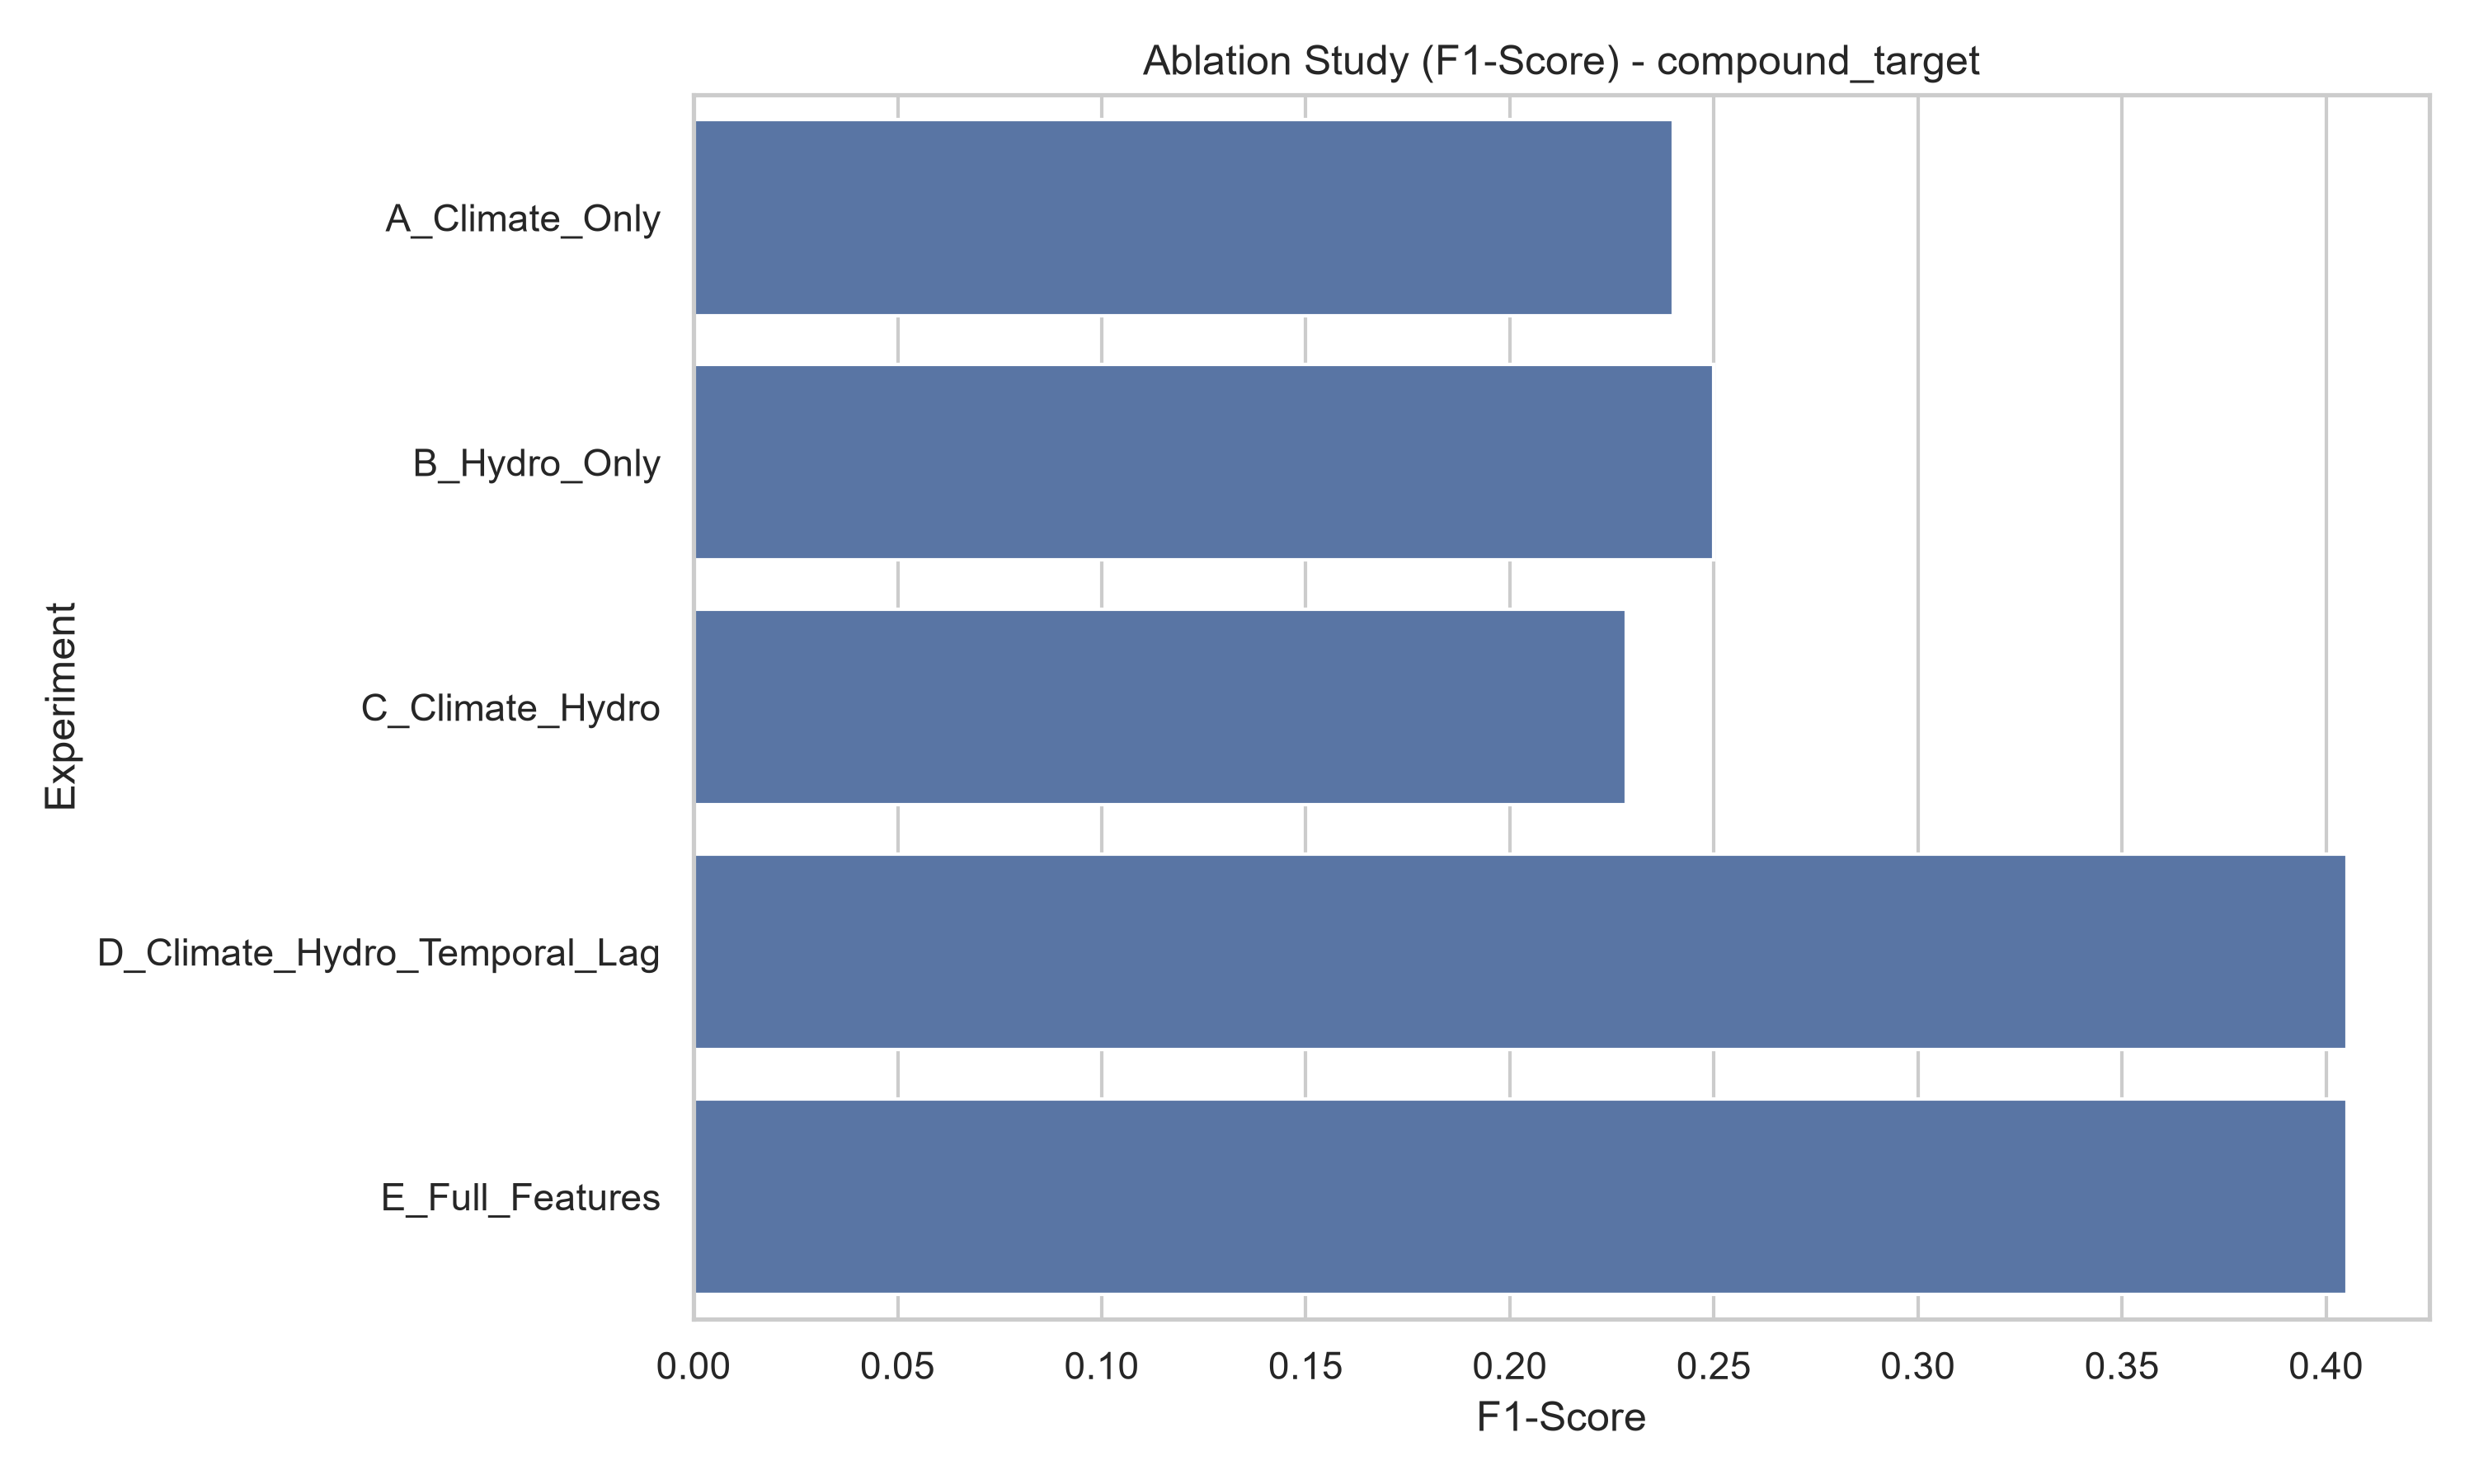
\includegraphics[width=\columnwidth]{figures/Fig07_Compound_Ablation.png}
\caption{Compound-risk ablation study showing the contribution of climate, hydrological, and temporal/lag feature groups.}
\label{fig:compound_ablation}
\end{figure}

\begin{table}[htbp]
\caption{FEATURE ABLATION RESULTS FOR THE COMPOUND-RISK TARGET}
\begin{center}
\resizebox{\columnwidth}{!}{
\begin{tabular}{lc}
\toprule
\textbf{Feature Configuration} & \textbf{Compound F1-Score} \\
\midrule
Climate Only & 0.2400 \\
Hydro Only & 0.2500 \\
Climate + Hydro & 0.2286 \\
Climate + Hydro + Temporal/Lag & 0.4051 \\
Full Features & 0.4051 \\
\bottomrule
\end{tabular}
}
\label{tab:ablation}
\end{center}
\end{table}

\begin{figure}[t]
\centering
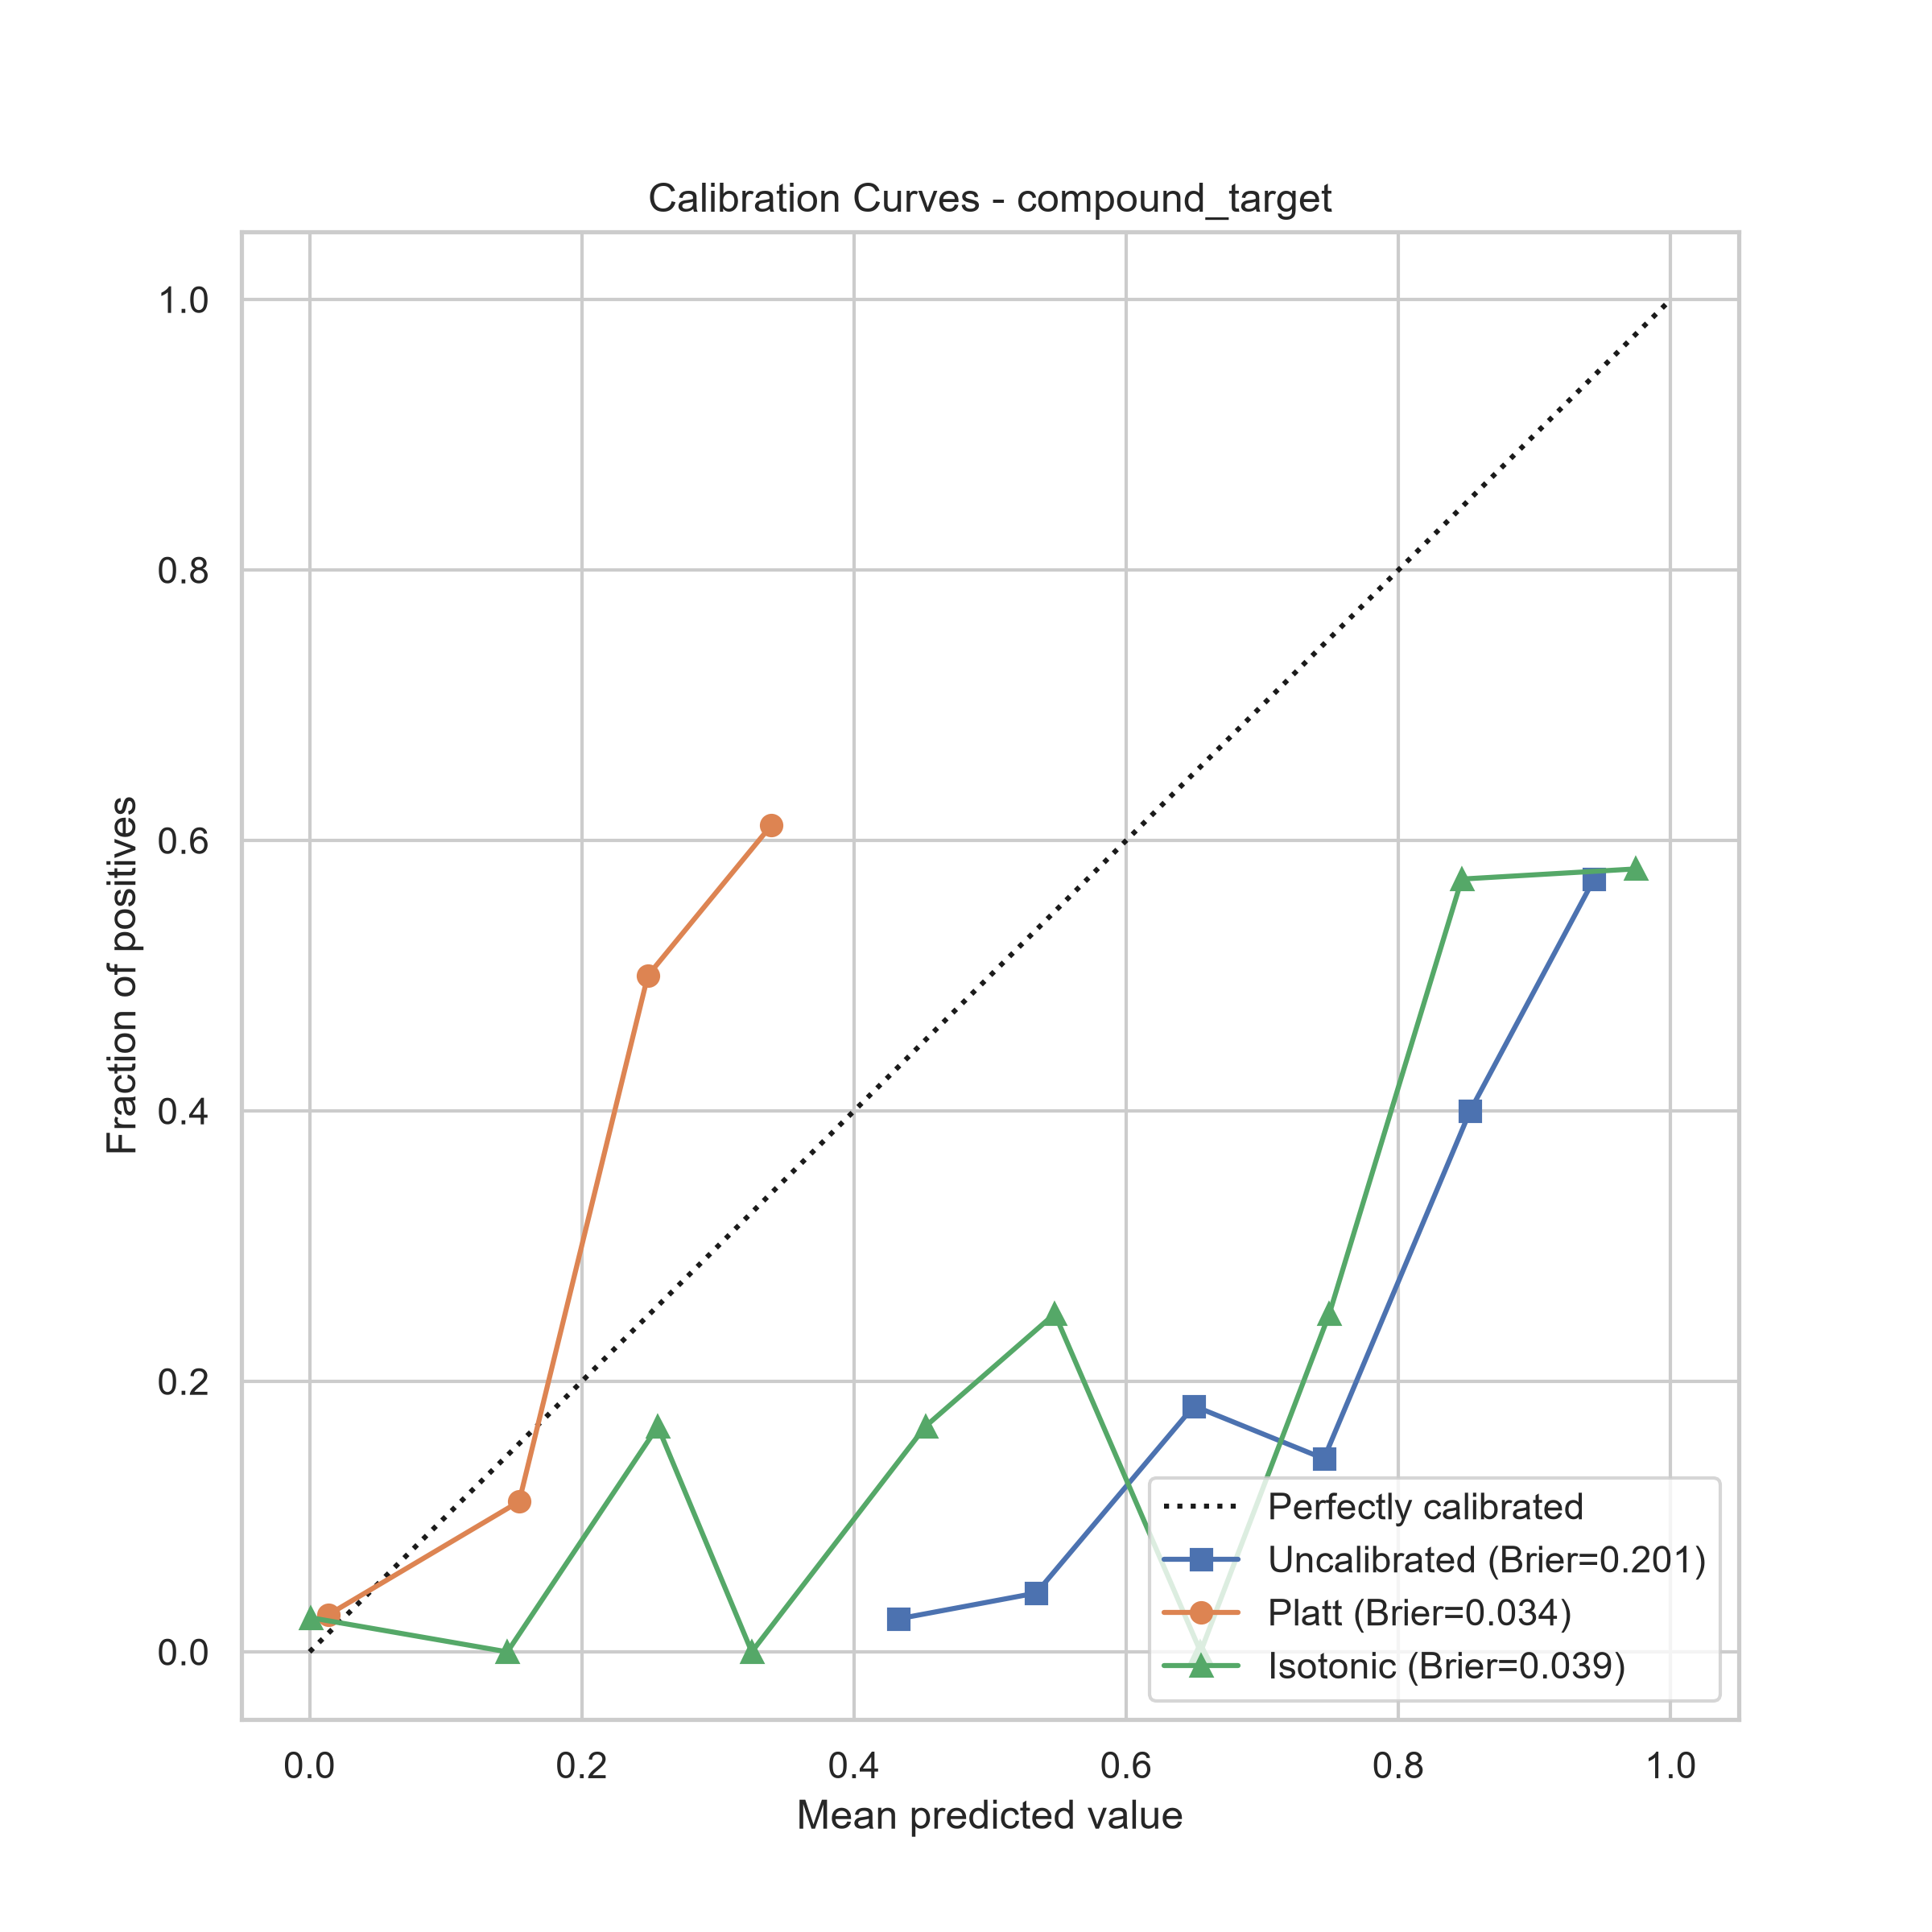
\includegraphics[width=\columnwidth]{figures/Fig04_Compound_Calibration.png}
\caption{Calibration analysis for the compound-risk prediction probabilities comparing uncalibrated, Platt-scaled, and isotonic-calibrated outputs.}
\label{fig:compound_calibration}
\end{figure}
To systematically determine optimal feature groupings, an ablation protocol isolated feature domains. The ablation results (Fig.~\ref{fig:compound_ablation} and Table~\ref{tab:ablation}) indicate that temporal and lagged information contributes substantially to Compound discrimination under the evaluated configuration. Evaluating isolated domains yielded lower Compound $F_1$ performance: Climate Only (0.2400), Hydro Only (0.2500), and Climate + Hydro (0.2286). However, integrating temporal and lag variables (Climate + Hydro + Temporal/Lag) resulted in a substantial relative performance increase to an $F_1$-score of 0.4051, matching the performance of the Full Features configuration (0.4051).

Parallel to classification discrimination, the reliability of probabilistic outputs was quantified using the Compound target (Fig.~\ref{fig:compound_calibration}). The uncalibrated baseline Brier Score of 0.2013 was compared against probabilities corrected via Platt Scaling (0.0338) and Isotonic Regression (0.0386). Under the evaluated calibration experiment, a lower Brier score indicates better probabilistic agreement, with Platt scaling producing the lowest verified Brier score among the evaluated approaches.

\subsection{Explainability and Overall Findings}

\begin{figure}[t]
\centering
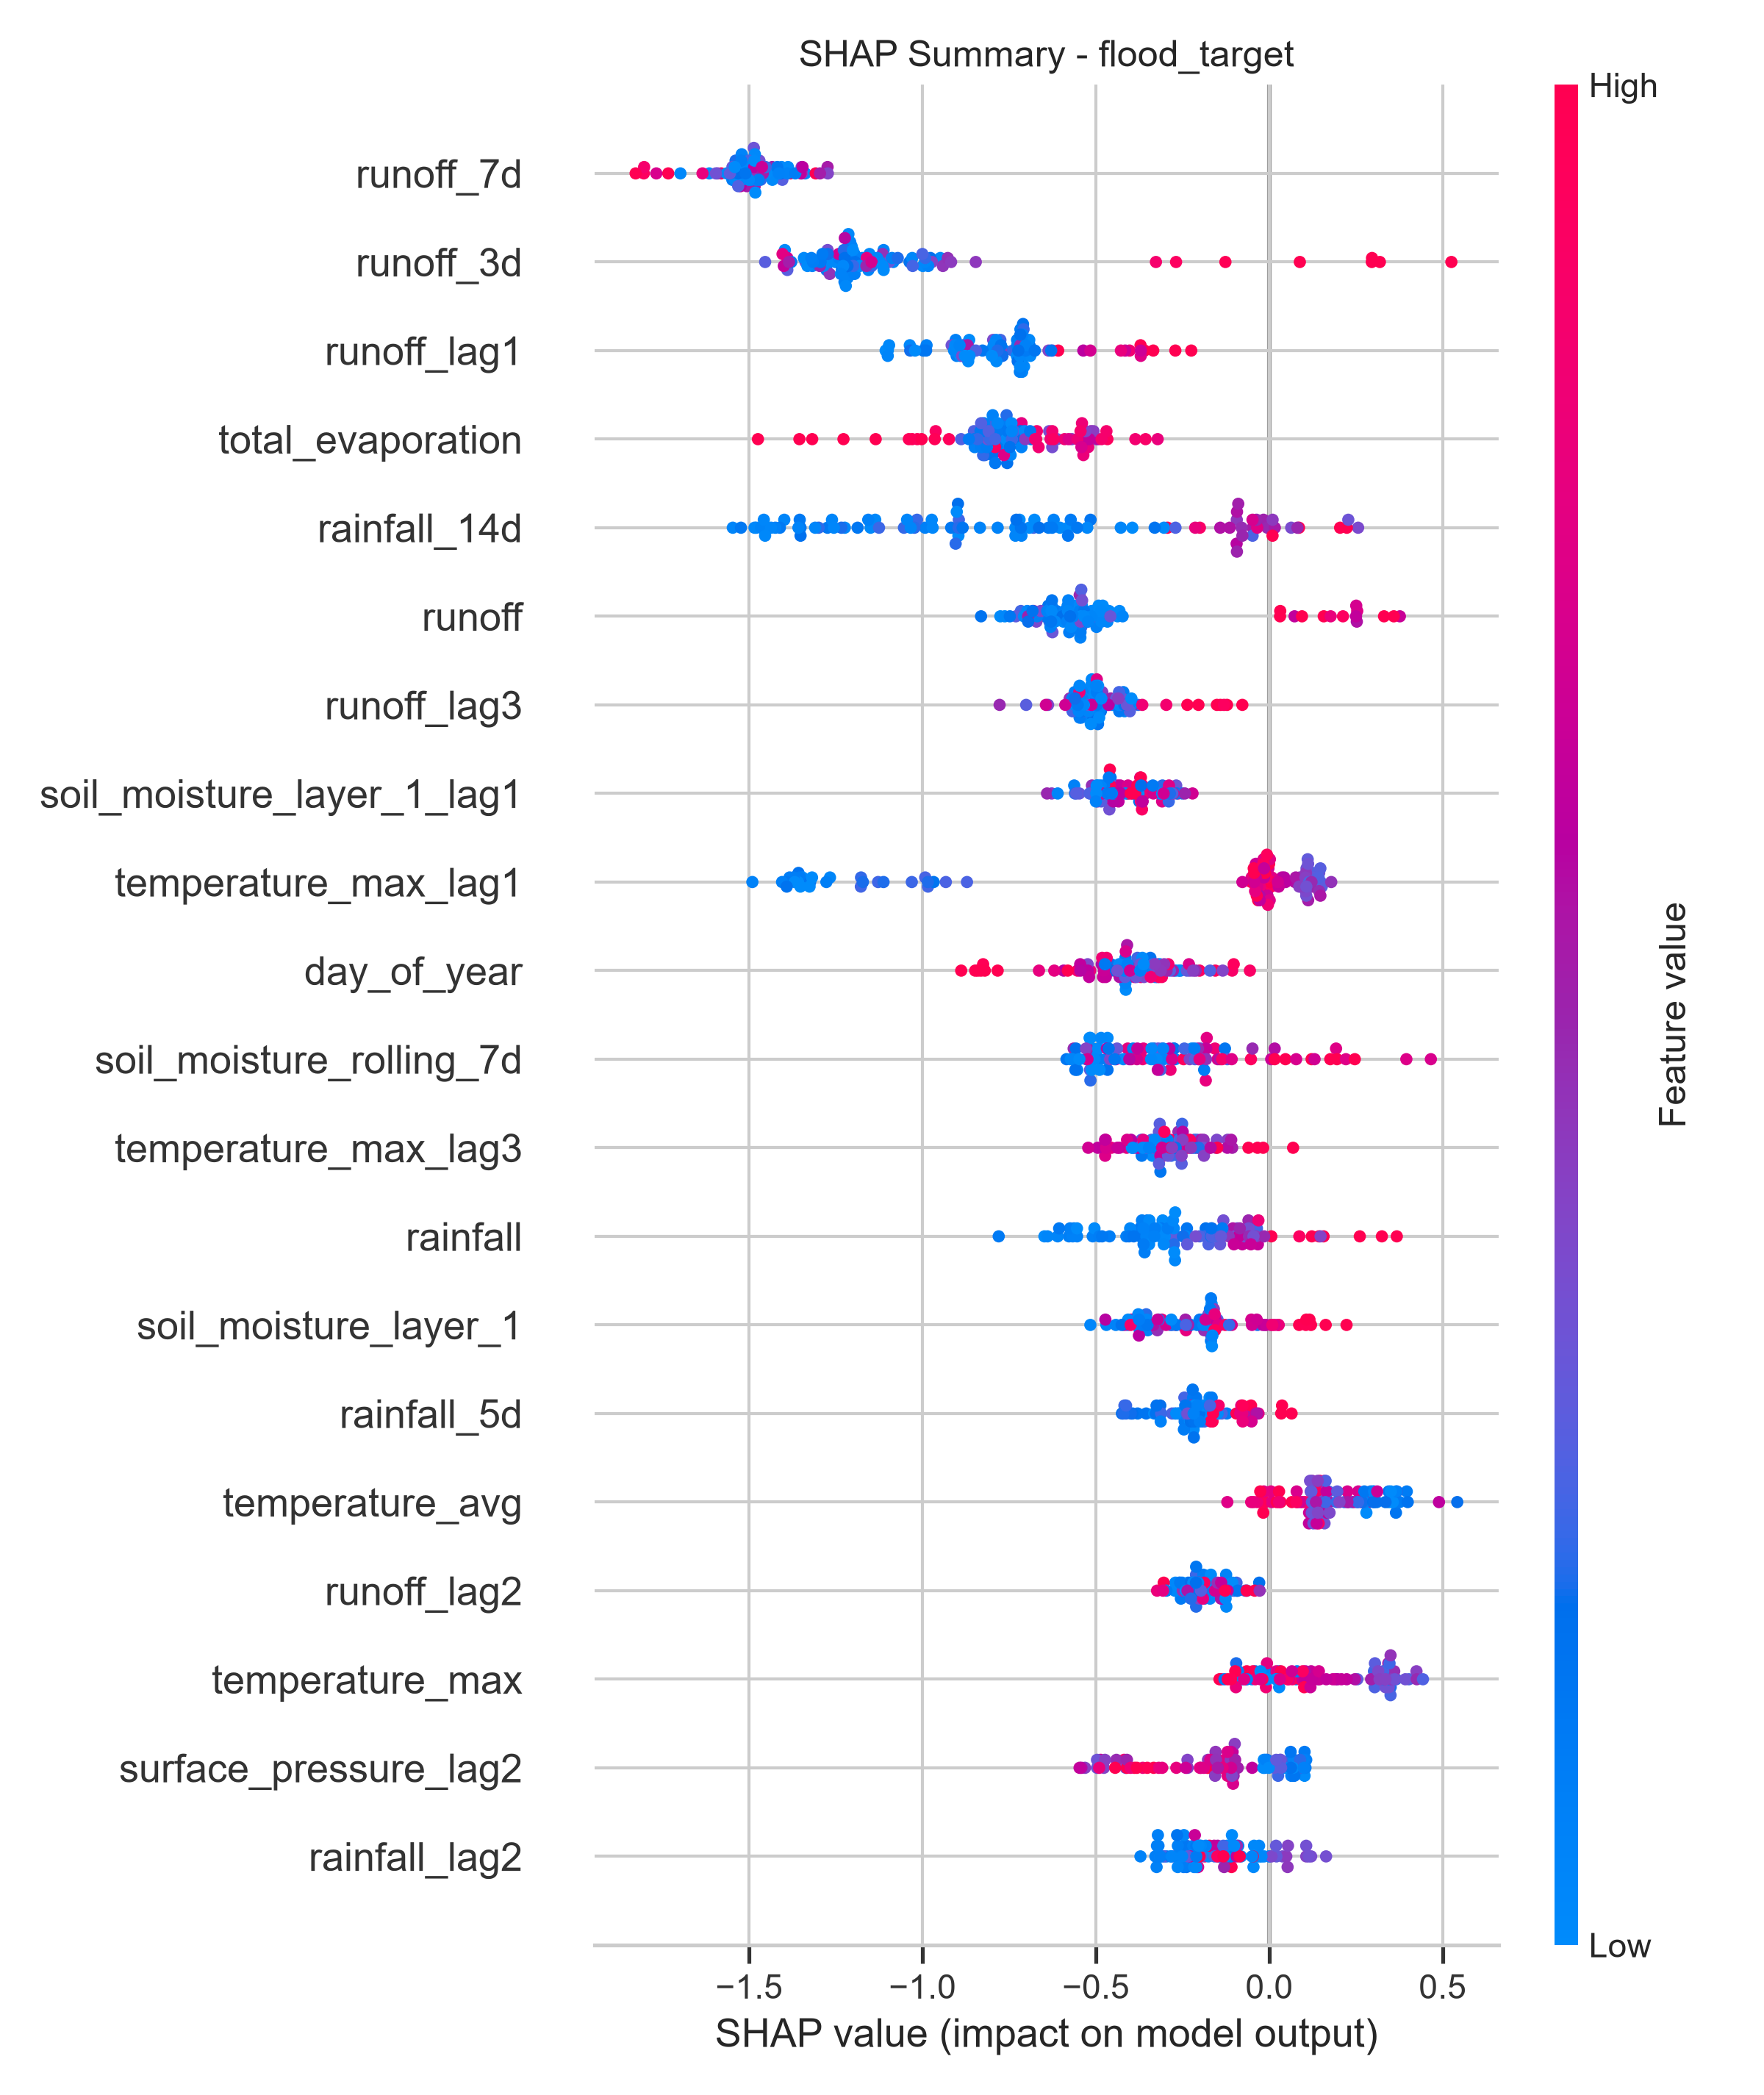
\includegraphics[width=\columnwidth]{figures/Fig05_Flood_SHAP.png}
\caption{SHAP summary of the Random Forest flood-risk model showing the internal feature-importance hierarchy.}
\label{fig:flood_shap}
\end{figure}
To interpret the internal dependency structure of the evaluated models, SHAP \cite{Lundberg2017} analysis was conducted (Fig.~\ref{fig:flood_shap}). SHAP provides insight into the internal feature attribution structure of the evaluated model by identifying the relative contribution of input features to specific predictions. Importantly, while SHAP characterizes model dependence, it does not establish physical causation.

Synthesizing the experimental evidence yields several supported findings. The selected Flood model provides moderate discrimination with relatively high recall compared with precision. The leakage-remediated Heatwave model retains strong predictive discrimination without the previously identified deterministic proxy features. The GRU provides the strongest verified offline Compound benchmark, yet the Stacking architecture is retained for operational prediction because its point-in-time architecture aligns with the stateless realtime pipeline. Temporally, Heatwave $F_1$ degrades with increasing lead time but remains measurable through 7 days, and temporal variables substantially improve Compound performance during ablation. Furthermore, Platt scaling calibration substantially reduces the evaluated Compound Brier score, and SHAP provides robust model-level interpretability without asserting physical causality.
